\documentclass{article}
\usepackage{fancyhdr}
\usepackage{tabu}
\usepackage[top=1in, bottom=1in]{geometry}
\usepackage{multirow}
\usepackage{graphicx}
\usepackage{setspace}
\usepackage{parskip}
\usepackage{pdfpages}
\usepackage{varwidth}
\usepackage{tocloft}
\usepackage{setspace}
\usepackage{hyperref}
\setlength{\parindent}{15pt}

\begin{document}
\noindent \begin{tabu} to \textwidth{l X[c] r}
\multirow{5}{*}{
\includegraphics[width=0.75in]{DOD.jpg}} & 
\textbf{United States Air Force Academy} &  
\multirow{5}{*}{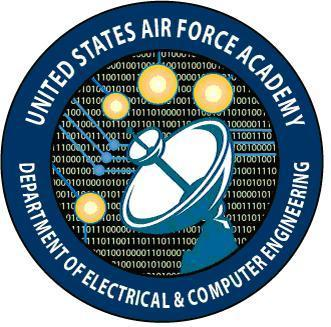
\includegraphics[width=0.75in]{DFEC}}\\
& \textbf{Department of Electrical and Computer Engineering} & \\
& \tiny{USAF ACADEMY, COLORADO}\\
\\ \\ \\
\end{tabu}

\title{Statement of Purpose}
\author{Ryan Silva, Captain, USAF\\Assistant Professor, Department of
Electrical and Computer Engineering\\United States Air Force Academy}
\date{}
{\let\newpage\relax\maketitle}

For as long as I can remember, I have been fascinated with how computers work
at the lowest levels and how hardware architects can overcome the
fickle nature of transistors as they become smaller and smaller. 
As an Air Force officer with over nine years of service, my career has largely consisted of
leading airmen in the application of a wide array of electrical and computer
engineering disciplines in operational and deployed environments. My most
recent assignment as a member of the United States Air Force 
Academy (USAFA) Faculty has afforded me the opportunity to impart my knowledge and
experiences to future generations of Air Force officers. Although my
experiences outside of USAFA were
intellectually stimulating, I want to state
unequivocally that my current position within academia has easily been the most
rewarding experience of my career and marks the genesis of my motivation to pursue
a Ph.D. 

As a graduate of both USAFA and the Air Force Institute of Technology
(AFIT), I have developed a set of core competencies that I believe make me well
suited towards doctorate level research. During my undergraduate years, I
participated in a multitude of embedded projects and developed competency in a
variety of hardware description and low-level languages, to include VHDL,
Verilog, and assembly languages for MIPS, S12, x86 and MSP430. I was
selectively chosen to participate in a cross-disciplinary
program where I successfully designed, implemented and optimized a
reconfigurable encryption architecture on a Field Programmable Gate Array
(FPGA) that I later applied to the Advanced Encryption Standard (AES) algorithm
in my graduate thesis. Immediately following my undergraduate studies, I was
awarded a graduate fellowship to study low-level computing and embedded systems
at the Air Force Institute of Technology. I focused my research on real-time
signal processing and communication theory using embedded systems culminating
in a novel method of implementing AES using an 8-bit datapath, implemented on
an FPGA. The resulting implementation and my findings were patented as an Air Force
Invention and awarded the Association of Old Crows Academic Research Excellence
Award, which came with a cash prize. In the course of my background research, I
began to understand the challenge current hardware architects face: as the size
of embedded processors and cores becomes exponentially smaller and the
computational demands grow exponentially higher, hardware becomes more and more
unreliable. I also learned that the current remedy to this issue, namely to add
more cores and processors in the name of parallelism, may not be the most
efficient and long-term solution to the original problem.

I became more aware of the increasingly unreliable nature of hardware after
graduating from AFIT and receiving my first non-academic assignment. While
stationed at the 84th Radar Evaluation Squadron (RADES), I was tasked with
reengineering the organization's largest and most complex legacy radar
monitoring system from the ground up. This requirement, part of
\href{http://en.wikipedia.org/wiki/Operation_Noble_Eagle}{Operation Noble
Eagle}, came in direct response to the attacks of September 11, 2001 and
required developing a hardware and software solution that integrated all
Federal Aviation Administration (FAA) radar sites into a single air picture.
Compared with the toy problems of academia, the technical challenges that I
encountered in the course of developing this solution seemed insurmountable.
Large quantities of data required processing in real-time and our existing
hardware just could not keep up, or worse, would provide erroneous results. The
existing solution to the problem was simply to add more hardware. A moment of
revelation occurred, however, when I
stopped concentrating on the quantity of hardware (scaling and parallelism) and
started focusing on the quality of the hardware as well as redesigning the
codebase with simplicity and efficiency in mind. The result was the squadron's
first real-time, reliable radar integration test tool.

The success of the RADES project was a turning point in my life, as it cast
aside my preconceptions of hardware design and introduced me to the notion that
massive parallelism in low-level and embedded computing may not be addressing
the bottleneck in the progression of processor design. This bottleneck has
grown out of the need to make hardware faster without making transistors
smaller. I realized that the key measures of success in achieving the above
goal are found in low-level hardware metrics, primarily minimizing power
consumption. Emboldened by my early achievements, I quickly discovered that
there are many aspects of hardware and embedded systems design that I never
considered. I realized that real-time signal processing could be better
realized through the implementation of simple algorithms executed rapidly and
reliably rather than through large, cumbersome computations that require a
watchdog for hardware and software faults. This realization paid dividends
during my sabbatical at the National Security Agency (NSA), where I was able to
deliver a solution to a critical shortfall in support of national security.
Using my newfound design mentality and deep interest in and knowledge of
embedded systems (primarily FPGAs) I was able to impress senior agency leaders
with the efficiency and reliability of my solution. I was suprised to discover
that the agency had awarded me \$10,000 in equipment and an additional \$10,000
for travel and incidentals to further hone my design. I later found out that my
solution, which I delivered in three weeks, solved a problem that had stumped
three full-time researchers for half of a year. 

The intellectual and creative challenges associated with designing efficient
low-level hardware architectures continue to intrigue me and I believe that my
background and experience in both hardware architecture and signal processing make
me uniquely suited to delve into these areas of study in greater detail.
Lincoln Labs agrees with my assessment as they have awarded me a
\href{http://www.ll.mit.edu/college/fellowsprograms.html}{Military Fellowship},
with full funding, to study these issues at a school in the Boston-area. With
this fellowship, I will represent a significant connection to Lincoln Labs that
is meant to foster collaboration with the university in the long term. I am
specifically applying to Harvard because of its reputation for excellence in
the fields of low-level hardware design. If accepted to Harvard, I would like
to conduct my research alongside faculty such as Professor David Brooks or
Professor Gu-Yeon Wei, as their work in low-level, power-efficient architecture
design aligns incredibly well with my interests and prior experience. While I
will return to the Air Force upon the successful completion of a Ph.D. program,
I envision myself as a lifelong researcher in the fields of low-level and
embedded computing. It is my hope that my work will influence the development
of future military and government systems, and that I will one day return to
USAFA to inspire future students to become the hardware savvy professionals
that our nation so desperately needs.


\end{document}
